\chapter{Intergroup bias in Reddit NFL game comments}
\label{chapter:football}

\begin{center}
    \textit{\textellipsis a socially acceptable outlet for xenophobia. That is the function of organized sports (in society) for the most part\textellipsis}
    \\\hspace{4em}---John Siracusa, \href{https://www.relay.fm/rd/3}{Reconcilable Differences Ep. 3}
\end{center}

Chapter~\ref{chapter:twitter} described my first data-driven study of intergroup bias in real-world language use, by curating a dataset of tweets by members of U.S. Congress with metadata derived gold labels for intergroup relationship. Crowd-sourced annotation revealed the systematic variation of interpersonal emotion with intergroup labels, and modeling further reinforced the systematic interaction between these two variables. In the previous chapter, I described my probing experiment to discover if the interaction between specificity and affect could describe any of the systematic \emph{linguistic} variation observed in the data. While the results were inconclusive, they were instructive towards how we needed to proceed towards answering this question --- we needed to look within utterances for intergroup variations in how people \textbf{referred} to the in-group and out-group, and we needed to \emph{tie} the variation in intergroup language to the events preceding the utterance.

As I have described earlier, the LIB hypothesis is limiting and ad-hoc towards capturing the rich forms of variation that we do observe in natural language. For instance, the dataset of political tweets was restricted to tweets where there was only one explicit referent (via @-mentions). However, the \textbf{form of referencing} the in-group or out-group can reveal subtle biases as well. Consider these tweets:

\ex. \label{ex:trump-tweets} \a.\label{ex:trump-tweet-1} \textbf{Mr. President}- Please tell your supporters to STAND DOWN, LEAVE the Capitol grounds and obey law enforcement who once again are risking their lives for our country!\textellipsis
    \b. \label{ex:trump-tweet-2} \textellipsis~Americans deserve answers on these unacceptable delays. We need a full accounting of \textbf{Pres Trump} and defense officials’ decisions on Jan 6~\textellipsis
    \b. \label{ex:trump-tweet-3} We survived an insurrection and \textellipsis~In we made it clear what St. Louis already knew: \textbf{Donald Trump} was the white supremacist-in-chief.

All of these tweets \emph{refer} to the same individual --- Donald Trump. However, \ref{ex:trump-tweet-1} is by a Republican Congresswoman (and thus in-group), while \ref{ex:trump-tweet-2} and \ref{ex:trump-tweet-3} are by Democrats (out-group). One can observe distinct changes in how the speakers \emph{refer} to him that is tinged by their (intergroup) relationships and changes in state-of-the-world. The Republican's tweet is more respectful, by only referring to him by position rather than name.  The LIB hypothesizes variation only in the form of the predicate --- this is an acceptable simplification when eliciting experiments in utterances, but discards useful information, as illustrated in these examples, in real-world language use.

To decipher the linguistic variables that underlie the systematic variation in the intergroup bias, we need to move beyond the political domain which suffers from two major drawbacks:

\begin{enumerate}
    \item A difficulty in succinctly describing the events in U.S politics immediately preceding the tweet.
    \item Much of the language by politician's is not natural speech by one person --- it is the output of a social media team who monitor many if not all of the tweets.
\end{enumerate} 

In this chapter, I introduce a new dataset of interpersonal language --- specifically sports comments from subreddits (internet forums) dedicated to fandoms for teams in the National Football League (NFL). As I will show, through careful data curation, we can obtain utterances with reliable information about the group allegiance of the writer of a comment (the in-group team they support), as well as a grounded score (the win probability) that describes the state-of-the-world (in a non-linguistic manner) prior to the utterance of a comment. Annotation and preliminary analysis reveals a crucial blindspot in the LIB --- the \emph{form of the referent} (the argument to a predicate) that speakers use when referring  to the in-group or the out-group may have systematic variations as well. By carefully exploiting the information processing capabilities of Large Language Models (LLMs), we can validate this systematic variation on a large-scale of over 200,000 Reddit comments spread over two years, revealing two striking social behaviors:

\begin{enumerate}
    \item The better the state of affairs in the real world for the \emph{in-group}, the more likely commenters are to \textbf{abstract away} from specifically referring to the in-group. This trend is remarkably linear across win probabilities for all types of in-group references.
    \item References to out-groups by commenters remain stable over all win probabilities for the in-group, with only a slight uptick in the frequency of referring to the out-group using names or nicknames when they are close to defeat or victory.
\end{enumerate}

These findings add much needed color to the LIB hypothesis --- natural language is productive, and commenters can express their (implicit) intergroup bias beyond the predicate; The form of the referent itself shows systematic variation in response to changes in the state of affairs for the in-group. This chapter is an account of my efforts in this direction. \textsection~\ref{sec:football-data} gives an overview of the dataset, the structure of the NFL, and the robust nature of the grounded variables readily available against comments. In \textsection~\ref{sec:football-prelim}, I detail the new protocol for tagging \emph{references} to the in and out-group at a lexical level, to create a new expert annotated set of comments tagged with intergroup labels. Then, I move on to describing my efforts building models that can effectively learn to tag words/phrases with intergroup tags on a large-scale(\textsection~\ref{sec:football-models}), which enables the statistical analyses and insights I derive in \textsection~\ref{sec:football-analysis}. I conclude in \textsection~\ref{sec:football-conclusion} with a discussion of the findings in light of intergroup bias more generally.

\section{A new dataset of interpersonal language}
\label{sec:football-data}

In Chapter~\ref{chapter:twitter}, I listed two conditions for the type of language we want to analyze for intergroup bias, restated here:

\begin{enumerate}
    \item Each utterance must have at least one target individual (person or group) about whom the utterance mainly concerns.
    \item The relationship between the speaker and the target must be inferred based on metadata or other information.
\end{enumerate}

These constitute \textbf{interpersonal} utterances. To these, we add another condition: a correspondence between each utterance and a \textbf{non-linguistic} description of the events that preceded (or precipitated) the events themselves. As I will show in this section, social media comments by fans of sports events, in particular the NFL, satisfy all of these conditions and offer a fertile ground for study.

\subsection{Prior work} 


Language use within the domain of sports has been a rich source of analyses and studies within computational linguistics, including from the perspective of quantifying \emph{social biases}. \citet{merullo-etal-2019-investigating} studied commentator racial biases in descriptions of football players, reaffirming previous findings illustrating clear differences in terms of sentiment descriptions (white players were more likely to be described as intelligent), and name itself (white players were more likely to be referred to by their first name). 

Human language learning and understanding does not happen in isolation; Indeed it is acquired and used in the physical world. Grounded language understanding aims to bridge the gap between the state-of-the-world, and the language that we use to talk about it~\citep{krishnamurthy2013jointly}. The sports domain is suitable for exploring the link between language and grounded descriptions of the world, as sports like football employ scoreboards, statistics, and constantly updated databases to accurately track the state of the game. The state-of-the-world of a football game at any moment can be described using the score, the team in possession, yards gained, yards left to opponent touchline, and previous plays up to that point. \citet{liang-etal-2009-learning} rely on such descriptions to build a generative model that maps from utterances (in a recap of the game) to state-of-the-world (generated from the scoreboard and database of events provided by the NFL).

While there has been a wealth of work looking into the language used around sports and sports commentary, our work differs from previous work in two major ways. Firstly, ours is the first study to focus on the intergroup bias (rather than race or other social factors) --- how do fans talk about their team, versus the opponent? Though sports as domain may seem trivial (as compared to politics, in our previous dataset), the insignificance of sports is precisely what makes studying human social-linguistic behavior in this realm interesting. People are less restrained speaking their mind freely, thus showcasing implicit (and explicit) prejudices freely~\footnote{as opposed to tweets by politicians (which are generally managed by social media teams) and commentators (who have to maintain an aura of neutrality, and obey broadcast regulations)}. Furthermore, \textbf{affective polarization is desirable} in sports for this very reason as well, whereas the rise of affective polarization has been studied extensively as a negative phenomenon in politics~\citep{iyengar_origins_2019}.


Secondly, this dataset (and the analyses that follow) studies the intergroup bias grounded in the events of the game parallel with the online comments. Social desirability was chosen as one of the axis of variation in the original LIB --- however, this is an ad-hoc formulation that is hard to generalize over and study at scale. Affect, as described in the previous chapter, was derived form the utterance itself rather than reflecting the state-of-the-world prior to the utterance. As I will explain, sports games, and in particular NFL football games, are rich with statistical information that allow us to describe the state-of-the-world on a numerical scale.

\subsection{Dataset} 

\paragraph{Data source for intergroup comments} Our new dataset of intergroup language comes from Reddit --- specifically subreddits (forums) dedicated to fandoms for each of the 32 teams in the NFL. During the NFL season, each subreddit has \emph{game threads} --- posts created by moderators on which fans can comment in tandem with the game. Crucially, since every subreddit has their own thread, we effectively have a \textbf{parallel} intergroup language corpus; we have two teams and their fans, each with different allegiances, commenting on \textbf{the same events in the game}. 

We focus on all completed games from 2021--22 and 2022--23 NFL seasons, and attempted scrape all comments from the game threads for both teams involved in every game. Furthermore, we also attempted to scrape comments from pre-game threads and post-game threads where available from subreddits. Table~\ref{tab:football-stats} gives summary statistics on our dataset after scraping. Within comments from game threads, we created a subset of comments that happened during active gametime --- which we label as \textbf{gametime} comments. Most threads are closed, or become inactive, once a game ends. Game threads are usually created (by subreddit moderators) and open for comment a few hours before the start of a game.

\begin{table}[t]
    \centering
    \begin{tabular}{lr}
        \toprule
        \textbf{Stat} & \textbf{Number} \\\midrule
        Teams & 32 \\ \midrule
        Games & 568 \\ \midrule
        Game threads & 1104 \\ \midrule
        Pre-game threads & 261 \\ \midrule
        Post-game threads & 1040 \\ \midrule
        Game thread comments  & 6,240,285 \\ \midrule
        Gametime comments & 6,679,988 \\ \midrule
        Pre-game thread comments &  \\\midrule
        Post-game thread comments &  \\\bottomrule
    \end{tabular}
    \caption{Summary statistics of our dataset. Game comments are judged to be game thread comments that happened \emph{during} the course of the corresponding NFL game. Comment timestamps were compared with publicly available start and end times of games.}
    \label{tab:football-stats}
\end{table}


\paragraph{Grounding football comments} As remarked earlier, one reason for studying intergroup bias in sports comments is the ability to \textbf{ground} the language in quantifiable descriptions of the state-of-the-world. NFL, and American Football in particular, has some attractive features as a sport considering that our interest is in the \emph{language} surrounding the events in the game. While physical, American Football is also one of the more strategic sports games, where outcomes are heavily dependent on a coach's strategies and plays in a (relatively) small number of discrete events~\citep{pelechrinis2016anatomy}.

There has been a wealth of work looking into predictive modeling of different statistics and events in a football game~\citep{horowitz2017nflscrapr, Yurko2018nflWARAR}, from predicting expected points scored by teams, to yards gained by individual players. The state-of-the-world at any moment in a football game is determined by a variety of factors --- the performance of teams before the game, the live score, the position of the offense, defense, and so many more. \citet{baldwin2021nflfastr} modeled the {Win Probability} (WP) of a team at any point during the game using the following features:

\begin{itemize}
    \item seconds remaining in half (and game).
    \item yard line
    \item score differential
    \item down, yards to go, timeouts remaining for each team
    \item whether team is playing at home
    \item Betting odds lines from Vegas
\end{itemize}

They find that simple decision tree based models with gradient boosting achieve a lower calibration error than previous models, and furthermore, incorporating the Vegas betting odds substantially reduced the error rate even further. For these reasons, we chose win probability (henceforth abbreviated as WP) as a succinct description of how desirable the state-of-the-world is to the in-group.

The NFL publicly releases play-by-play information after every game, which includes details on the plays and the timestamp of each play. The \texttt{nflFastR} package includes WP for the home team alongside each and every play, updating it as the game state evolves with each play. In concert with the comments (whose timestamp of submission we also have access to), we can thus derive the WP for the in-group at the time of the comment by selecting the WP for the most recent play at the time the comment was made. The WP for the away team is simply set as 1 minus the WP for the home team. 

Table~\ref{tab:football-exs} lists some comments from the 2023 Super Bowl between the Chiefs and the Eagles, with the win probability for the Chiefs in the middle. As is evident, the WP cleverly models the complexities of a real-world sporting event into one number that accurately models how \emph{desirable} the state-of-the-world is to the in-group. This a marked improvement on \emph{social desirability} as an axis in the LIB, which was ad-hoc, and \emph{affect} in our previous formulation, which was derived from the utterance rather than from the state-of-the-world.

\begin{table}[t]
    \centering
    \begin{tabular}{lcl}
        \toprule
        \textbf{Chiefs fans comments} & \textbf{Chiefs WP} & \textbf{Eagles fans comments} \\ \midrule
        Now I’m nervous…. & 0.25 & Good shit covey \\ \midrule
        Oh, is there a defense on the field? & 0.75 & Burn that clock baby \\ \bottomrule
    \end{tabular}
    \caption{Comments from the Chiefs subreddit(left), and the Eagles subreddit(right) with the WP for the Chiefs in the middle. The WP for the Eagles is 1-WP for the Chiefs.}
    \label{tab:football-exs}
\end{table}
 


\section{Tagging \& Annotation}
\label{sec:football-prelim}

The tweets in \ref{ex:trump-tweets} illustrated a phenomenon that the Linguistic Intergroup Bias failed to account for --- systematic variation in how people refer to the in-group versus the out-group. Moreover, our prior method of classifying the utterance(tweet) as a whole was too coarse to capture some of the variation observed in our original dataset, that we discarded due to the assumption of at most one \@-mention target. A preliminary analysis of our scraped data illustrate the problem with this approach:

\ex. \label{ex:mult-football} \a. \label{ex:mult-football-a} Rams are gifting us a chance to win and we can’t take advantage. The fuck!!!!
     \b. \label{ex:mult-football-b} if the ravens and chiefs beat these dudes by double digits then damn it so should we!
     
Even without contextual information for the above comments, we see a few different references to entities that we can readily identify as references to the in-group, out-group, and perhaps another category adjacent to the out-group. These examples suggest an alternate framing, or approach to modeling, of \emph{references} to entities that are in-group or out-group, based on pre-existing tasks and pipelines in NLP: tagging.

\subsection{Tagging in-group vs. out-group}

Instead of judging an utterance as a whole to be primarily about the in-group or the out-group, we concern ourselves with how individuals are \emph{referred} to in interpersonal comments themselves. The words or phrases that refer to the individuals can now be tagged with in-group([IN]) or out-group([OUT]) For instance, the examples in \ref{ex:mult-football} could be \textbf{tagged} thus:

\ex. \a. [OUT] are gifting [IN] a chance to win and [IN] can’t take advantage. The fuck!!!!
     \b. if [OTHER] and [OTHER] beat [OUT] by double digits then damn it so should [IN]!
     
     
In both sentences, we find that we can readily identify some words and phrases as references to the in-group with respect to the commenter --- like the first person plural pronouns \textbf{\emph{we}} and \textbf{\emph{us}}. This is a common expression by sports fans to express affinity towards their in-group as highlighted in the language of these comments.

The spans `Rams' in \ref{ex:mult-football-a} and `these dudes' in \ref{ex:mult-football-b} are clear references to the \emph{out-group} with respect to the commenter --- one can come to these inferences with some reasoning over the choice of words by the commenter, verified further by knowledge of the source of the comments, and the live score. The spans `the ravens' and `chiefs' in \ref{ex:mult-football-b} is more interesting --- it is clearly not a reference to the in-group nor the opponent of the game. However, it is a reference to \textbf{a group of interest in this domain} --- another NFL team and/or its fans. We consider these references to be [OTHER], and a special case of out-group references.

Tagging words and phrases within comments with their intergroup tags enables us to study utterance-level properties (how are people talking about the in-group and out-group), as well as how commenters choose to refer to the in-group and out-group themselves. However, to discover whether there are systematic differences in how commenters refer to and talk about groups, and the interaction therein with world-state(WP), we need a large, diverse sample of comments in our original dataset tagged. To build robust models for tagging comments with intergroup tags, we need a well annotated dataset of sufficient size and sample diversity. For this purpose, we construct a detailed annotation protocol with examples, which is described in the following section.

\subsection{Annotation Protocol}

Annotators are presented with a comment from our dataset, and some context from the state-of-the-world using a browser based interface. They are given the following high-level instructions:

\begin{enumerate}
    \item All comments are from game threads corresponding to specific NFL games between two teams. You will be given the source of the comment --- this is the team the writer of the comment supports, the opponent in that game, and the live score at the time of making the comment.
    \item Highlight any words and phrases that refer to individuals (people, teams, sub-groups within the team, organizations).
    \item If the reference is to the same group as the source subreddit of the comment, tag this highlight as \textbf{in-group} ([IN]).
    \item If the reference is towards the opponent in this specific game for which the comment is written, tag this highlight as \textbf{out-group} ([OUT]).
    \item If the reference is towards any other team in the NFL apart from the two teams involved in this game, tag this highlight as \textbf{other} ([OTHER]).
\end{enumerate}

The task of tagging words and phrases from comments in our dataset with intergroup tags can be highly involved, as the following examples show. In addition to knowledge of American Football, commonsense reasoning over the meaning of an utterance in context of the state-of-the-world (live score), one needs knowledge of the teams and players. For instance, in the following comment, one needs to know that the commenter supports the Seahawks, and that there is a prominent player named Wilson, to accurately tag in context that Wilson indeed is an in-group reference.

\ex. Our oline should start holding since apparently it ’s okay now . Maybe Wilson can actually get some time to throw .

In other instances, the references to the in-group, out-group or other are not as explicit. However, we can infer based on context, and state-of-the-world (live score or WP), that the comment as whole, or a sentence in the comment, is \textbf{implicitly referring} to the in-group/out-group/other. Consider this example:

\ex. Lets go to the 4th with a 1st down around midfield.

There is no explicit word/phrasal reference to any team in the above comment\footnote{\emph{lets} was originally a contraction of \emph{let us} which has the first person plural pronoun.}. However, it is clear that the commenter is referring to the in-group --- such an expression or admonition to the out-group or any other team would not be phrased in such a way. To facilitate these implicit annotations, we append a sentence-level token [SENT] before each sentence, and ask annotators to highlight and tag this sentence-level token if they believe the sentence as a whole is implicitly referential to a group. These annotations require a higher bar of reference, since all the comments are about the game at hand and will involve both teams to some extent. For instance, the following comments, we judge to not have explicit or implicit references to any relevant groups of interest (and label them as \textbf{null referent} comments henceforth):

\ex. \a. Fair enough !
     \b. winning cures all lmao
     \b. turning the game off , have a good day yall
     
In case it is impossible to verify an explicit or implicit reference, annotators are instructed to not highlight any parts of the comment. While reasoning and information access (through team databases and search) can help in tagging several comments in the annotated dataset, pilot experiments revealed that a small fraction of comments are extremely hard to annotate, without onerous research into the events of the game and the live game thread. All annotation experiments were carried out using the \texttt{thresh.tools} annotation interface~\citep{heineman2023thresh}.

\paragraph{Expert annotated gold dataset} Due to the difficulty and involvement of this particular annotation task, we decided to rely on expert annotations for constructing a `gold' annotated dataset. I personally annotated 1499 comments (randomly sampled from \emph{game thread} comments) for intergroup references based on the protocol above. Some preliminary statistics of the annotated dataset are presented in Table~\ref{tab:test-football-stats}. 26.7\% of this random sample were judged to have no relevant intergroup reference, and in the remaining comments, references to the in-group vastly out-number references to the out-group or other groups. This is not surprising, since these are comments from forums dedicated to fandom of teams --- people are much more likely to talk about their team over the opponent. This compliments our finding in Chapter~\ref{chapter:twitter} of in-group tweets being overwhelmingly positive.

\begin{table}[t]
    \centering
    \begin{tabular}{lr}
        \toprule
        \textbf{Stat} & \textbf{Number} \\\midrule
        Game threads & 768 \\ \midrule
        Games & 491 \\ \midrule
        Comments  & 1499 \\ \midrule
        Comments with no annotation & 399 \\  \midrule
        Number of <in> annotations & 1393 \\\midrule
        Number of <out> annotations & 266 \\\midrule
        Number of <other> annotations & 166 \\\bottomrule
    \end{tabular}
    \caption{Summary statistics of expert annotated gold test set.}
    \label{tab:test-football-stats}
\end{table}


\subsubsection{Annotation Results \& Analysis}

To understand the annotation process better, and understand individual variation in what `counts' as a reference to the in-group and out-group to be tagged, we recruited annotators for a crowd-sourced annotation experiment. This annotation experiment has two goals --- gauge inter-annotator agreement among crowd annotators and sources of disagreement, and identify  who operate under stricter constraints of time (and impoverished knowledge of the task and dataset) 

\paragraph{Inter-annotator agreement} To evaluate the reliability of collecting annotations for intergroup labels using the protocol above, we ran a small pilot study over a sample of 100 comments from the gold dataset. 3 annotators (undergraduates) were recruited to perform annotations, and presented with the same annotation protocol that I used to construct the gold annotation dataset. Average Fleiss $\Kappa$ among these 3 annotators is  0.65, indicating moderate agreement.

In addition to the inter-annotator score, by counting exact-matches and weighting partial matches between individual crowd annotators and gold annotation, we calculate a score of $0.71 \pm 0.03$. This gives a human upper bound for performance on this task, and characterizes its inherent subjectivity and difficulty.

\paragraph{Disagreement or diversity?} Inter-annotator agreement among annotators, as well as the averaged accuracy of crowd-annotators against gold annotations, were both found to be in the moderate-to-high range of values. While this lends credence to the annotation protocol and the task design, looking at the source of disagreements can give us insights into the nature of the task itself, as well as why differences in judgements of intergroup affiliation can come down to annotator biases or judgement given context~\citep{atwell-etal-2022-role}, as well as implicit thresholding on what counts as a `reference', as these examples demonstrate:

\ex. \label{ex:disagree} \a.\label{ex:disagree-a}\textellipsis of the assorted ballparks and stadiums and concert venues I've been to , \textbf{Lambeau} has the second worst bathrooms .
    \b. \label{ex:disagree-b} Can’t do that against \textbf{an offense} this good.
    \b. \label{ex:disagree-c} Let ’s go baby

\emph{Lambeau} in \ref{ex:disagree-a} was judged to be a reference to the out-group in the context of this utterance --- which was from the Colts subreddit in a game against the Green Bay Packers. However, to disambiguate this reference, annotators would need to know (or search to discover) that Lambeau Park is the stadium in which the Green Bay Packers play, and furthermore make a judgement call that this constitutes a relevant intergroup reference. As the expert annotator, I judged that it was a reference to the out-group because I discovered through search the relevance of \emph{Lambeau} to the out-group. 

In addition to requiring time and multiple steps of search and reasoning on the part of the annotator, the disagreements between annotators (and between annotators and gold annotation) illustrate variations in the implicit threshold of what constitutes an intergroup reference. For instance, \emph{an offense} in \ref{ex:disagree-b} was judged by some annotators to refer to the out-group in context (the in-group was losing), however the generic nature of the referent lead some annotators to judge that this was an overall statement about the game, rather than a reference in of itself. Similarly with \ref{ex:disagree-c}, some annotators judged the comment as a whole to be about the in-group (boosting or building them up) based on context and commonsense reasoning; However, other annotators judged this to be an expression of excitement by the fan, and not an obvious reference. 

\paragraph{Is disagreement a signal of intergroup bias?} Overall, these findings and examples paint a complex picture of how to reconcile agreement between annotators, and disagreements that nevertheless provide reliable signal towards the intergroup bias. Whether or not examples in \ref{ex:disagree} contain references to the in/out-group is not simply a consequence of the difficulty of our task, or the inability for annotators to transparently describe the mental state of commenters (which we also observed annotating for interpersonal emotion as described in \textsection~\ref{subsec:twitter-annotation}). Rather, we need to analyze them as possibly another subtle influence of the intergroup bias itself --- demonstrated by posing the question as to why annotators chose the forms in \ref{ex:disagree} rather than in \ref{ex:disagree-alt}, which seemingly convey the same meaning, and would be uncontroversial in annotation:

\ex. \label{ex:disagree-alt} \a. \textellipsis of the assorted ballparks and stadiums and concert venues I've been to , \textbf{the Packer's} stadium has the second worst bathrooms .
    \b. Can’t do that against \textbf{the Packers} offense this good.
    \b. Let's go \textbf{Packers}!

The intergroup bias can observed to lead to subtle shifts in reference form, as we will see in forthcoming sections. However, future work needs to look into embracing the inherent annotation diversity in this task with grounded context, which can boost model performance on involved tasks that require linguistic and commonsense reasoning over world knowledge and context~\citep{atwell-etal-2022-role}.

\subsection{Qualitative Analysis \& Trends}
\label{subsec:football-trends}

The annotated dataset enables us to study qualitative trends, that will guide quantitative modeling and regression studies presented in \textsection~\ref{sec:football-analysis}. I want to specifically focus on two phenomenon that are directly observable in the data and illustrated with examples --- diversity in form of referring expression, and trends over WP.

\begin{figure}[t]
    \centering
    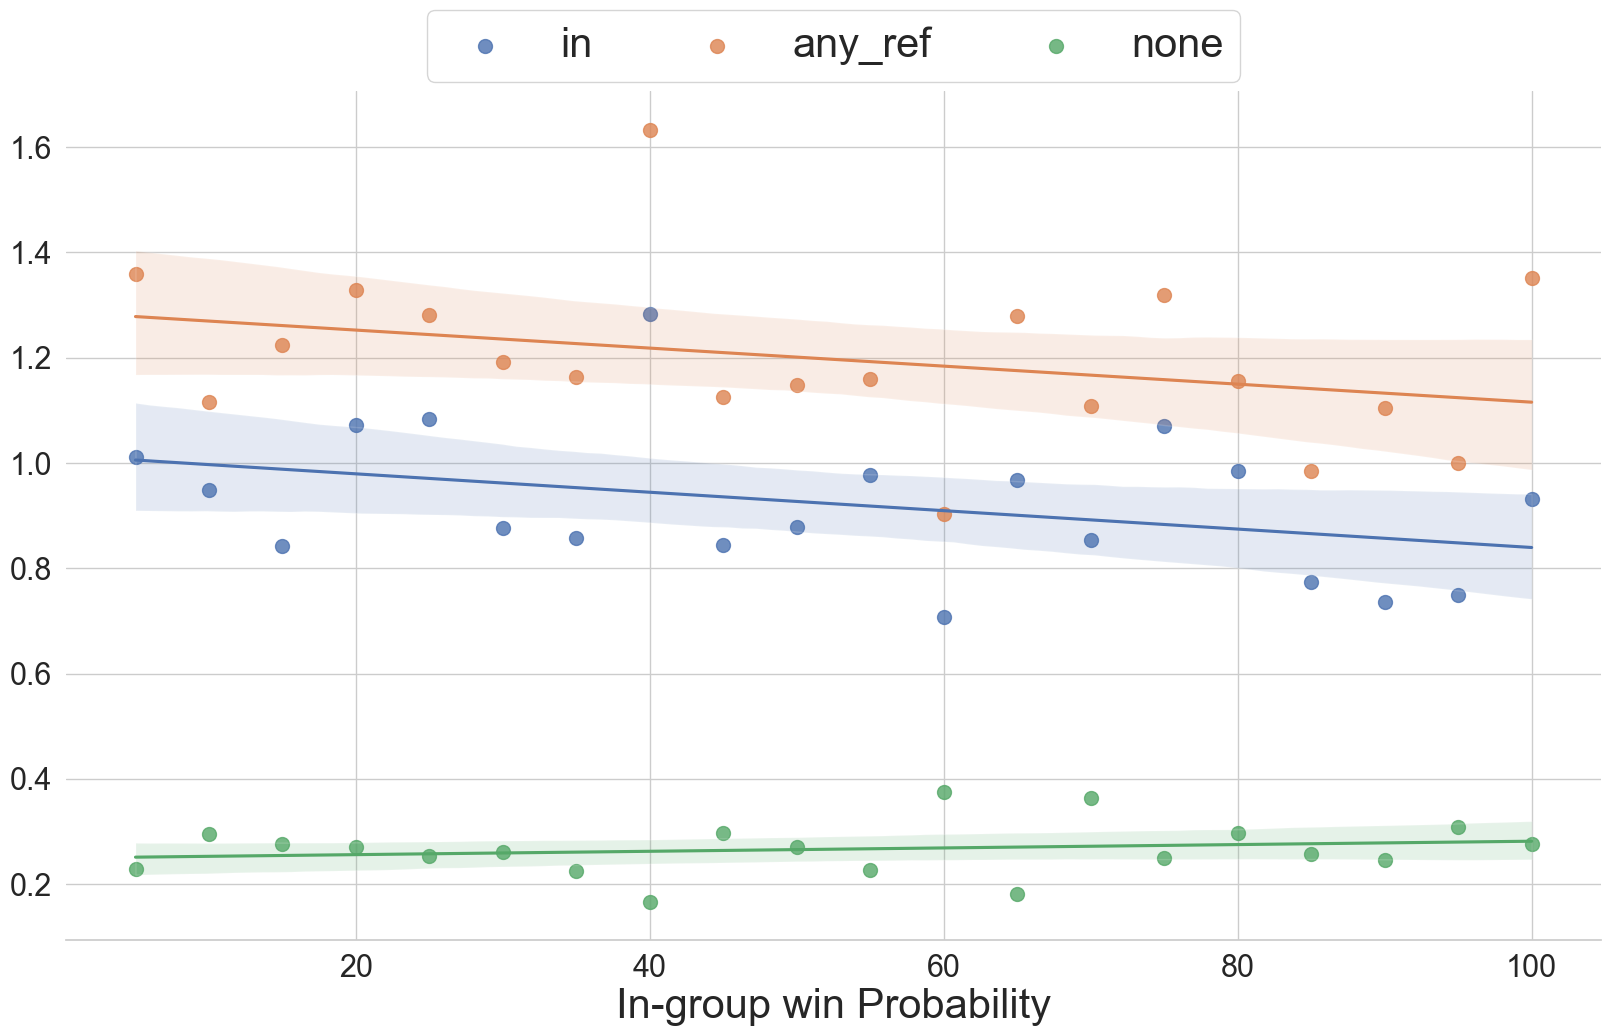
\includegraphics[width=\linewidth]{figures/test-trends.png}
    \caption{Frequency of any-group, in-group and null references in comments that fall in 5\% WP windows from 0 to 100. A simple regression line with 95\% CI is fit separately for each feature to show some noisy trends.}
    \label{fig:test-trends}
\end{figure}

\paragraph{Mereology of referring expressions} Expert annotation revealed that commenters refer to groups of interest in a myriad of different ways. In the previous section, we liberally defined the annotation protocol for highlighting references to \emph{individuals} in the in-group, out-group and other. Using insights from mereology~\citep{sep-mereology}, I derive a taxonomy of `parthood' in intergroup relations, that defines what it means for a reference to constitute a reference towards the in-group/out-group/other:

\begin{enumerate}
    \item \textbf{Names of people}: Commenters frequently refer to individual players and coaches using names, nicknames, shirt numbers, initials, pronouns, etc. : \emph{Tua, TK87, he/him\textellipsis}
    \item \textbf{Subset of the team}: This refers to groups of players, or coachers, rather than just one player: \emph{the offense}, \emph{our defense}, \emph{o-line}, \textellipsis
    \item \textbf{Team}: This is the standard way of referring to the team, but there is a host of variety within this category as well. In addition to the name of the team (\emph{rams, bills, cowboys}), nicknames (\emph{lambs, cowgirls}), city names(\emph{LA, Buffalo, Dallas}), commenters also use pronominal expressions like \emph{our boys} for the in-group, pronouns like \emph{they/them} for the in-group and out-group, and many more.
    \item \textbf{Team plus supporters}: This is the largest possible reference to the in-group/out-group. References to the in-group generally involve the first person pronouns \emph{we} and \emph{us}, but can also be done with the third person pronouns \emph{they} and \emph{them}. The latter of course, could also refer to out-group or other, and require contexts to disambiguate.
\end{enumerate}

The taxonomy above is ordered ad-hoc in order of increasing coverage of the whole group, by the referential part --- the size of the reference gets larger from people to the entire group. Thus, players are the smallest unit of reference within a group, and the team/organization plus its supporters constitute the largest possible reference to the group itself. However, there are diverse ways of referring to each group within each, as the examples above illustrate.

\paragraph{Trends} Within this expertly annotated dataset, we can observe two clear trends by plotting the frequency of a feature of interest over comments that fall within a win probability (WP) window. Figure~\ref{fig:test-trends} plots the frequency of any reference (in-group, out-group or other), in-group references, and null references over all WP probabilities:

\begin{enumerate}
    \item References to the in-group, and references to any group overall, clearly go down with win probability.
    \item Null references steadily with increasing WP for the in-group.
\end{enumerate}

The steady increase in number of null references in higher WP windows is interesting, and seem to be attributable to a combination of euphoria at being close to victory, and a tendency to abstract away from specific gametime events to be terse and celebrate the victory, as the following examples show.

\ex. \a. I can't stop smiling!
     \b. Absolute domination!
     \b. ITS COMING BACK!

While the trends observed in this section are not statistically or practically significant (the slopes in Figure~\ref{fig:test-trends} are small), this can be attributed to the small sample size of analysis. Our expert annotated dataset is only 1500 comments. The intergroup bias is a social phenomenon, and like many social phenomenon, we can make clear inferences at scale (CITATION). Obtaining human annotated data at scale would be prohibitively hard and expensive in this setting --- thus, we turn to fine-tuning Large Language Models, to automate this task, thus allowing us make inferences about trends in the intergroup bias as a function of WP. The next section will also give us insights into the difficulty of training large machine learning models on the difficult task of \emph{tagging} words and phrases in comments with their intergroup referential tags.

\section{Modeling the Intergroup bias with LLMs}
\label{sec:football-models}

Large Language Models (LLMs) have shown remarkable abilities in various domains over the last few years~\citep{Brown2020LanguageMA}. LLMs trained on next-token prediction score highest on numerous benchmarks: from linguistic understanding~\citep{srivastava2023beyond}, knowledge and search~\citep{geminiteam2023gemini}, to complex reasoning~\citep{NEURIPS2022_9d560961}. Recent very large language models exemplify \emph{in-context learning} (ICL) behaviors as well. Rather than finetuning on specific tasks, ICL relies a few training examples (few-shot) fed into the model prompt at inference time, effectively ``learning'' via inducing internal activations of the LLMs in such a manner as to pre-dispose it to perform well at the task.

As I've shown in the previous section, annotating comments from our dataset to highlight spans that refer to the in-group, out-group or other requires linguistic understanding, knowledge of the NFL and its teams, as well as complex reasoning over why a commenter might choose certain word forms compatible with the state-of-the-world --- LLMs excel at all of these. Can we use LLMs to automate tagging of comments in our dataset with intergroup references? Consider the following example, with information about the in-group w.r.t the commenter, the out-group (opponent), and the win probability at the time of making the comment:

\begin{verbatim}
    COMMENT: If we could combine Pickett 's underthrows with
    Mariota 's overthrows , we'd get a pretty good QB.
    IN-GROUP: Falcons
    OUT-GROUP: Steelers
    WP: 0.12
\end{verbatim}

The first person plural pronoun \emph{we} should be annotated as in-group --- a model trained to tag comments on our dataset must learn that fans use \emph{we} to signal their group membership and fandom. There are two proper names denoting players; A model resolve the last names to specific players, figure out the team they play for, and thus tag the names respectively with the correct tags. The model could also reason over the structure of the sentence and the aligned WP, and figure out that Pickett is probably a member of the out-group, while Mariota is probably in-group, since the commenter wants to pick and choose qualities from another player to help with their own team's performance while they are losing. The final output should be of this form:

\begin{verbatim}
    TAGGED COMMENT: If [IN] could combine [OUT] 's underthrows with 
    [IN] 's overthrows , [IN]'d get a pretty good QB.
\end{verbatim}

This is a complex task, and for this reason we design a modeling approach that aims to exploit the capabilities of LLMs to the fullest extent possible, and understand which techniques serve us best towards tagging on a large scale. We focus on finetuning an off-the-shelf Instruction-tuned encoder-decoder language model \texttt{Flan-T5-Large}~\citep{Chung2022ScalingIL} specifically for our task, and analyze the impact of instructions, few-shot examples, and explanations on the task of tagging comments with intergroup tags.

\subsection{Model types}

\texttt{Flan-T5-Large} is an encoder-decoder model --- the encoder encodes the input prompt, upon which the decode learns to attend to different regions of interest, when generating its output, token by token. Thus, our task is framed end-to-end as taking the untagged comment with contextual information (in-group, out-group, WP), and it is asked to generate the comment with relevant words/phrases replaced with the appropriate tags. For instance, here is a sample training input:

\begin{verbatim}
    COMMENT: [SENT] Defense getting absolutely bullied by a dude
    that looks like he sells solar panels
    IN-GROUP: Jets
    OUT-GROUP: Bears
    WIN PROBABILITY: 71.5%
    TARGET:
\end{verbatim}

and here is the model's expected output after the word TARGET:

\begin{verbatim}
    [SENT] [IN] getting absolutely bullied by [OUT] that
    looks like [OUT] sells solar panels .
    REF_EXPRESSIONS: ['Defense', 'a dude', 'he']
\end{verbatim}

In addition to the tagged comment, the model is trained to generate a list of the referring expressions that have been tagged in the original comment (for ease of analysis later).

In general, performance of LLMs has scaled with compute and data in recent years~\citep{kaplan2020scaling}. However, the best LLMs are prohibitive to use in academic research settings due to cost and resources. Finetuning \texttt{Flan-T5} by itself solely on our gold dataset with the above format leads to poor performance by itself, since our training dataset is small. However, we can bolster its performance by incorporating a few different techniques: 

\begin{description}
    \item[Few-shot] To facilitate ICL, we prepend 5 examples (not from our gold dataset) with the above training datapoint format to each datapoint in our training data. This gives implicit demonstrations to the model of the behaviors we want it to learn.
    \item[Instructions] We prepend a short paragraph of text, giving instructions on how to perform the task, similar to the protocol we provided annotators. This is to further guide the model's ICL activations towards learning the tagging behavior correctly.
    \item[Explanations] Chain-of-Thought (CoT) prompting~\citep{NEURIPS2022_9d560961} has been shown to elicit complex reasoning for LLMs, by giving the model's a larger scratchpad and guiding model activations further towards desired behaviors. While CoT has generally been observed in extremely large models beyond the scope of this study, ~\citet{Wadhwa2023RevisitingRE} show that finetuning with CoT explanations generated from a larger model improves performance on relation extraction. We append a small explanation to the few-shot examples that explains why the comment ought to be tagged in this manner, and generate explanations for all datapoints in our gold dataset. The model is thus tasked to generate an EXPLANATION after REF\_EXPRESSIONS.
\end{description}

To generate explanations for all datapoints in the dataset, we use \texttt{gpt-3.5-turbo}, which we prompt with instructions and few-shot examples with explanations appended. Here is an example of a GPT generated explanation for the training example at the beginning of this section:

\begin{verbatim}
The commenter is likely a fan of the Falcons, as they are playing 
against the Steelers and have a low win probability. The comment is 
criticizing the quarterback play of both teams, mentioning 'Pickett' 
(Steelers) for underthrows (tagged as [OUT]) and 'Mariota' (Falcons) 
for overthrows (tagged as [IN]). 'we'd' should also be tagged as [IN] 
since it refers to the in-group, the Falcons.
\end{verbatim}

GPT-generated explanations involve complex reasoning over the entities mentioned in the comment, knowledge of football, as well as linguistic reasoning. Thus, while our model is relatively small \footnote{768M parameters, compared to GPT-3.5's 175B parameters}, we can still gain the advantages of CoT through finetuning on GPT-3.5 generated explanations.

\paragraph{Ceiling performance} To compare the effectiveness of our techniques, we also evaluate the performance of GPT-3.5 and GPT4~\citep{achiam2023gpt} on our gold dataset. We present each datapoint from our dataset with instructions, few-shot examples and explanations, asking the model to generate an explanation, a list of referring expressions, and the target tagged comment in that order.

\paragraph{Evaluation \& Implementation} Based on the techiques defined above, we build and compare 4 different fine-tuned models that explore different combinations of techniques: \texttt{fewshot}, \texttt{fewshot+instruct}, \texttt{fewshot+cot}, and \texttt{fewshot+instruct+cot}, where \texttt{+} indicates a combination of 2 or more techniques described above. We partition our gold dataset into a test set of 318 datapoints, and a training set of 1181 datapoints. 

To evaluate the performance of a model on the test dataset, we employ two forms of metrics:

\begin{itemize}
    \item We calculate \textbf{micro-F1} scores for each of the tags across the whole test set. Sometimes the model accurately tags the correct word/phrase, but is off by 1-2 characters/words. For this reason, we weigh each true positive match: if it is within one character of the gold tag's location, we assign a full correctness score of 1, if it is within 3 characters, a score of 0.5, and if it is within 5 characters, a correctness score of 0.25.
    \item We calculate two automated metrics that compare two sequences and generates the --- GLEU score~\citep{napoles-EtAl:2015:ACL-IJCNLP} and word error rate (WER)~\citep{woodard1982}. The former was designed for evaluating grammatical error correction, while the latter is analogous to edit distance. Both metrics are suitable for our task, where we want to penalize large amounts of differences between model generated tagged comments and the gold comments, while copying over most of the input comment.
\end{itemize}


\subsection{Results}

\begin{table}[t]
    \centering
    \begin{tabular}{lrrr}
        \toprule
        \textbf{Model} & \textbf{F1} & \textbf{WER} & \textbf{GLEU} \\ \midrule
        \texttt{fewshot} & 56.9 & 5.5 & 88.5  \\ \midrule
        \texttt{fewshot+instruct} & 54.0 & 5.2 & 88.1  \\ \midrule
        \texttt{fewshot+cot} & 54.5 & 5.3 &  88.1  \\ \midrule
        \texttt{fewshot+instruct+cot} & 60.0 & \textbf{4.9} & \textbf{89.8}  \\ \midrule
        \texttt{gpt-3.5-turbo} & 48.4 & 16.2 & 72.6  \\ \midrule
        \texttt{gpt-4} & \textbf{60.6} & 7.4 & 86.4  \\ \bottomrule
    \end{tabular}
    \caption{micro-F1 score (higher is better) over all tags, WER (lower is better) and GLEU scores(higher is better) on test split for all models.}
    \label{tab:results-football}
\end{table}


Table~\ref{tab:results-football} shows the overall results on all fine-tuned models as the GPT models. We observe that the model employing a combination of all of our techniques performs best overall, beating GPT-3.5, a model 2 orders of magnitude bigger, and is on-par with GPT-4\footnote{rumored to be a Mixture of 8 Experts each 175B in size}. The automated metrics reveal that each additional technique on top of few-shot examples reduces error ever so slightly, with the \texttt{fewshot+instruct+cot} model performing best in both automated metrics and tagging accuracy.

\paragraph{Copy errors} The low performance of the GPT models on the automated metrics is a function of low performance on copying behavior. GPT-3.5 and 4 need to copy most of the input comment over with small changes only over words and phrases to be tagged. Due to the non-deterministic and stochastic nature of these models, they make small errors in copying behavior --- missing some words, adding new words, changing tense/aspect of other words. Fine-tuning leads to much lower errors in copying.

\paragraph{Low recall} Table~\ref{tab:football-results-rec} presents the per-class recall performance of all models, illustrating the shortcomings of the fine-tuned models as compared to the much larger GPT-3.5 and GPT-4. GPT-3.5 and 4 perform better than our fine-tuned model on recall primarily for \textbf{tagging out-group references}, where our fine-tuned models overgeneralize towards tagging proper names as in-group (or not tagging it at all) due to the tag imbalance in our training data. GPT-4 correctly tagged the bolded names in the following examples as out-group, with the generated explanation also correctly citing 

\ex. \a. The fact that we dont have 10 sacks is just a testament to \textbf{Josh Allen}.
     \b. Anyone have a clip of the hit on \textbf{Huntley} ?

\begin{table}[t]
    \centering
    \begin{tabular}{lrrr}
        \toprule
        \textbf{Model} & \textbf{[IN]} & \textbf{[OUT]} & \textbf{[OTHER]} \\ \midrule
        \texttt{fewshot+instruct+cot} & \textbf{66.6} & 32.1 & 14.1 \\ 
        \texttt{gpt-3.5-turbo} & 54.5 & 39.3 & 32.1  \\
        \texttt{gpt-4} & 62.5 & \textbf{53.6} & \textbf{28.8}  \\ \bottomrule
    \end{tabular}
    \caption{Recall scores for each tag on test split for all models.}
    \label{tab:football-results-rec}
\end{table}


Is the model's performance affected by win probabilities? To ensure the analyses that follow are not an artifact of the model's weakness on comments from certain win probabilities, we verified that there was no correlation between the model's performance and win probability.

\section{Large-scale analysis of model tagged comments}
\label{sec:football-analysis}

In \textsection~\ref{subsec:football-trends}, we observed a clear intergroup bias over state-of-the-world (WP), however the significance of these findings were hampered by the same size of our hand-annotated data, and the expense of scaling towards tagging more comments. Our best fine-tuned model performs extremely well at tagging references to the in-group; while its performance on out-group (and other) references is low, the low-recall is uniform across win probabilities. Thus, the analyses presented in this section are still demonstrative of subtle manifestations of the intergroup bias on real-world language use, that could previously not be described by the LIB.

For the following analyses, we sampled over 223,680 comments from game threads, specifically focusing on \textbf{gametime comments}. We used the best performing \texttt{fewshot-instruct-cot} model to generated tagged comments, as well as the list of referring expressions and their corresponding intergroup tags. To mitigate some errors in copying and displacement, we performed edit checks between the tagged comment and the original comment so that the list of referring expressions was valid. In addition, we performed heuristic based tagging on top of the tagged comments from the model for first-person plural references using \emph{we/us}, as well as common names and nicknames for teams.

\paragraph{In-group trends}

\begin{figure}[t]
    \centering
    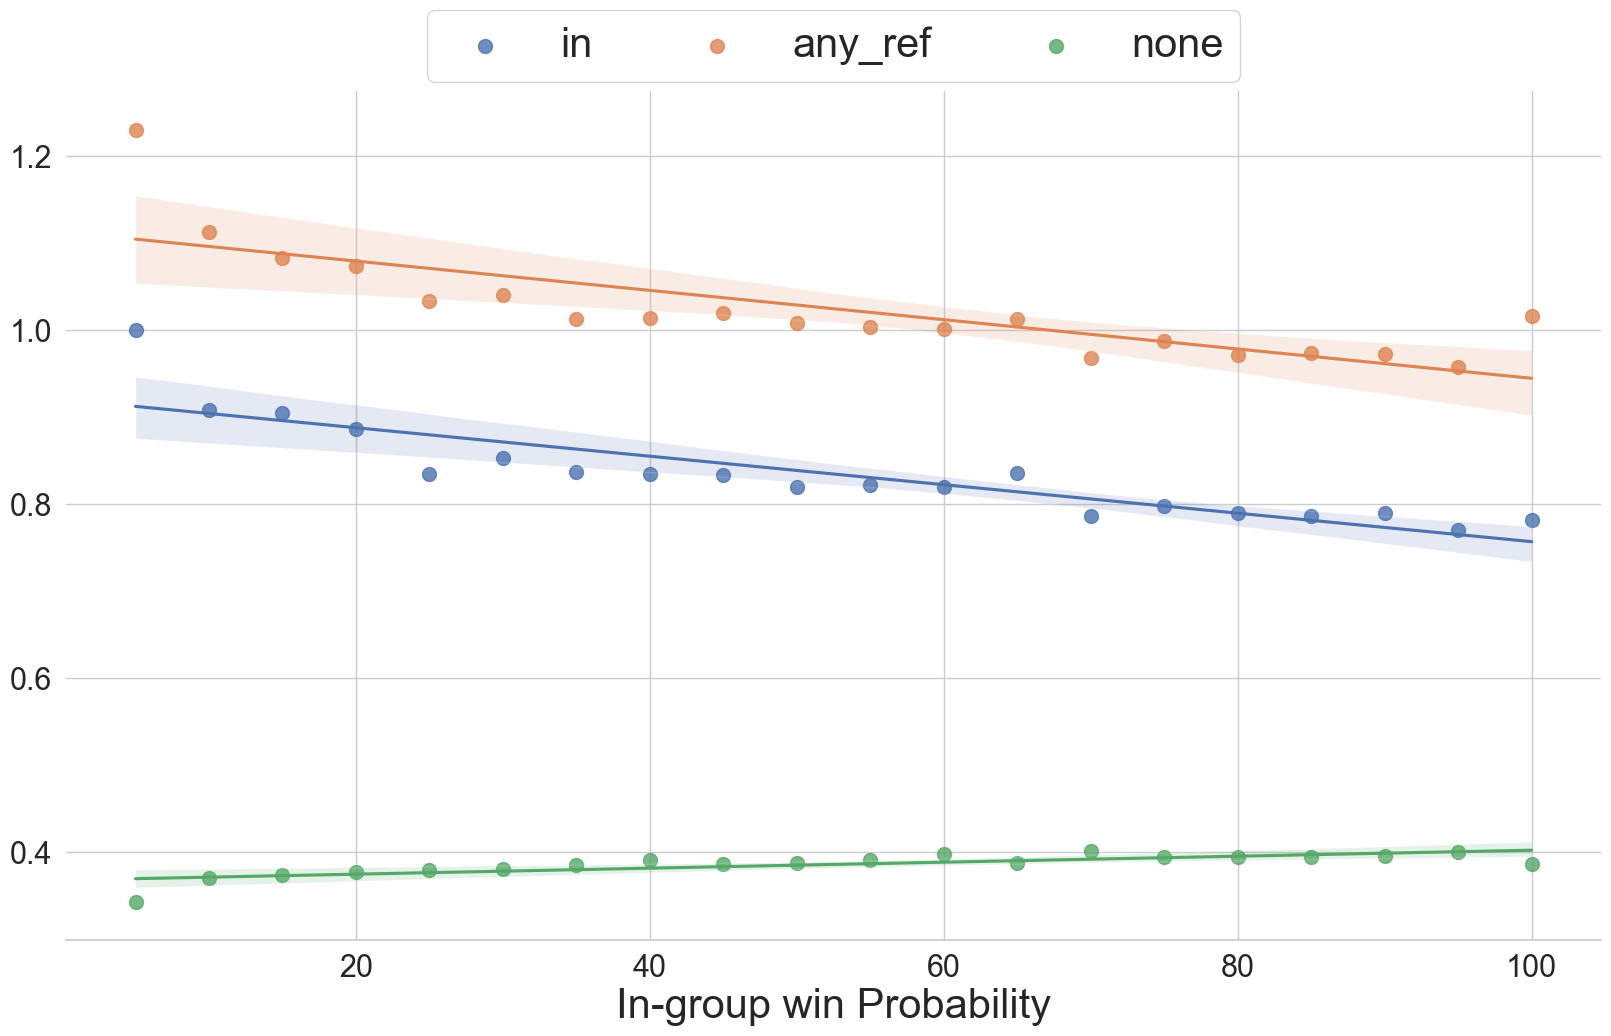
\includegraphics[width=\linewidth]{figures/trends-1.png}
    \caption{Frequency of any-group, in-group and null references over all 5\% WP windows from 0 to 100. A simple regression line with 95\% CI is fit separately for each feature to show clear linear trends.}
    \label{fig:trends-1}
\end{figure}

Figure~\ref{fig:trends-1} plots the frequency of occurrence of in-group, any-group and no references within each win probability window. Within, each win probability window, we count the occurrence of a variable of interest, and normalize it by the number of comments within that window. As the figure shows, there is a steady decline in the frequency of references overall, and in-group references (which constitute the bulk of references as established). The trend is surprisingly linear in its behavior, with outliers at the lowest, and highest win probability windows, where deviations in linguistic behavior by commenters might be expected, due to the certainty of winning and losing respectively.

\begin{figure}[t]
     \centering
     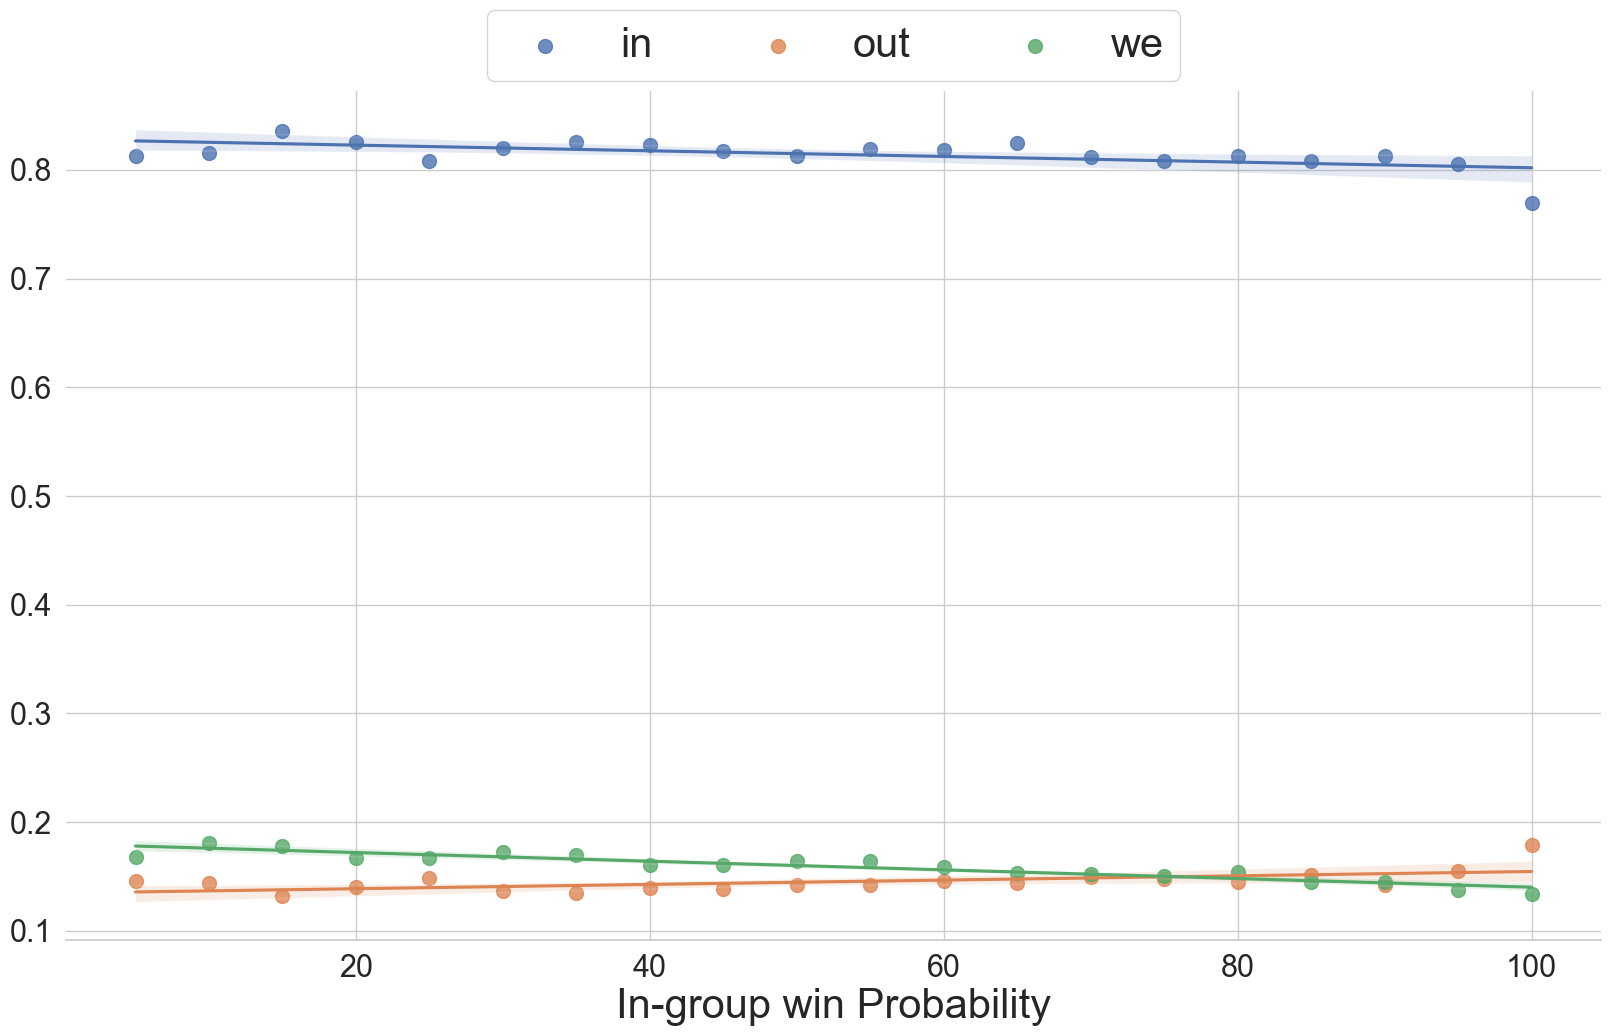
\includegraphics[width=\linewidth]{figures/trends-2.png}
     \caption{Frequency of references to the in-group using \emph{we/us} or \emph{they/them} over all 5\% WP windows from 0 to 100. A simple regression line with 95\% CI is fit separately for each feature to show clear linear trends.}
     \label{fig:trends-2}
 \end{figure}

Concurrent with the decrease in references is the increase in comments with no references to any relevant group. A cursory analysis of high WP(see~\ref{ex:high-wp}) and low WP(see~\ref{ex:low-wp}) comments with no references reveals an obvious increase in positive sentiment, but also increased terseness closer to victory. Comparing the length of comments, we find a very small but significant ($\rho=-0.05$ ($p<0.005$)) negative correlation between length of comment and the win probability.

\ex.\label{ex:high-wp} \a. HOLY SHIT 
     \b. DO NOT TAKE YOUR FOOT OFF THE GAS
     \b. WHAT A THROW
     
\ex.\label{ex:low-wp} \a. Lol like a preseason game.
     \b. Yeah I ’m done for tonight
     \b. Bruh ...

\begin{table}[t]
    \centering
    \begin{tabular}{lrr}
        \toprule
        \textbf{Feature} & \textbf{Slope} & \textbf{r-squared} \\ \midrule
        Any reference & $-17\times 10^{-4}$ & $0.61$ \\ 
        No reference & $3.5\times 10^{-4}$ & $0.57$ \\
        In-group & $-2.6\times 10^{-4}$ & $0.31$ \\ 
        \texttt{we} & $-4\times 10^{-4}$ & $0.87$ \\  
        out-group & $2\times 10^{-4}$ & $0.33$ \\
        in-group names only & $-2\times 10^{-5}$ & 0.04 \\
        out-group names only & $1\times 10^{-4}$ & 0.58 \\
        \texttt{they\_in} & $-4\times 10^{-5}$ & 0.22 \\
        \texttt{they\_out} & $6\times 10^{-5}$ & 0.33 \\ \bottomrule
    \end{tabular}
    \caption{Table of slopes of feature of interest against increasing WP, alongside the r-squared showing how much of the variance is explained by the linear regression fit.}
    \label{tab:slopes}
\end{table}


Overall, this seems concurrent with the idea that the better the state-of-the-world is for the in-group, the less likely commenters are to refer to the in-group in any form. Commenters are more likely to abstract away from referring to the in-group (or out-group) using explicit or implicit mentions, towards general expressions of sentiment or descriptions of the game itself (like in ~\ref{ex:high-wp}).
    
Figure~\ref{fig:trends-2} plots the frequency of references to the in-group using \emph{we/us} and \emph{they/them} (and their inflections) over all WP. While the frequency of \emph{we/us} decreases in line with overall in-group reference frequency, the slope is much lower. Table~\ref{tab:slopes} shows the slopes of a linear regression fit between the feature of interest and WP, showing that \emph{we/us} reduces at half the rate of overall in-group references. The prevelance of referring to the in-group using \emph{they/them} is much lower overall, and also goes down with increased WP as expected.

\section{Discussion \& Conclusion}
\label{sec:football-conclusion}

There are two takeaways from the application of our best fine-tuned model on a large, representative sample of our dataset. First, is the \textbf{linear and inverse} relationship between the frequency of references to the in-group and the state-of-the-world (win probability --- WP). Second, and concomitant with the previous finding, is the relatively stable association between frequency of out-group references and WP, and the \textbf{marked increase} in non-referential comments with increases in WP. We shall discuss both of these findings and their implications towards the intergroup bias in turn.

\paragraph{In-group} Figures~\ref{fig:trends-1} and \ref{fig:trends-2} display a remarkable linear relationship between two parameters that are operationalizations of the different aspects of the world. What does the decrease mean in context of this domain, and what is the significance of its linearity? This finding adds further evidence that not only is WP an accurate description of a complex state of affairs in football games, it is sufficient to capture a large amount of variation in linguistic behavior. In addition to being well calibrated as a machine learning model as described in ~\citet{baldwin2021nflfastr}, these results show that it is also well calibrated to \textbf{human appraisals of the state-of-the-world}. Through well devised `scoreboards' based on non-linguistic variables of interest, this gives us hope that similar simplified scores can be calculated to describe the state-of-the-world in non-sporting domains, towards replicating these findings in conversation more generally.

The trends observed with in-group references versus WP also add to the subtle ways we perpetuate bias in our linguistic behavior, especially in this case towards \textbf{in-group preservation}~\citep{maass_linguistic_1999}. While commenters are more than willing to criticize the in-group across WP, the self-protective instinct is evident in the way they choose to refer to the in-group using \emph{we/us} rather than \emph{they/them}, or to not refer to the in-group at all, abstracting away to talking about their sentiment or description of the events. How commenters choose the form of reference to an in-group constitutes just as subtle a bias as their choice of predicate.

\paragraph{Out-group} Regarding the out-group (and other), reference frequency remains stable over all WP --- commenters also refer to the out-group explicitly or implicitly much less. References to the out-group are most frequent at the lowest/highest WP (corresponding to the end of a game when win/loss is certain) and relatively stable throughout otherwise (see Appendix~\ref{appendix:figs} for plots). This is similar to our findings in Chapter~\ref{chapter:twitter}, where there was a clear bias in positive emotions towards the in-group, revealing a drawback of studying intergroup bias on naturally occurring language (as opposed to elicited utterances generally in the LIB) at scale --- speakers prefer to talk about their in-group overall, and with negative affect when they do talk about the out-group.

\paragraph{Modeling Improvements} As discussed in the previous section, there is room for improvement on large-scale tagging of referential expressions, especially out-group references. This doesn't detract from our analysis in the previous section --- the model's performance isn't correlated with WP, and a significant reason for the low performance of our model can be attributed to size. GPT-4 outperforms our model on recall over out-group references, and a lot of its gains come courtesy of its size. A new generation of open LLMs including Mistral~\citep{jiang2023mistral}, Gemma~\cite{geminiteam2023gemini}, and OLMo~\citep{Groeneveld2023OLMo} provide competitive performance on benchmarks to GPT-4, and exhibit complex reasoning and general knowledge of events and entities --- crucial towards performance on our tagging task. These need to be explored for further gains on out-group tagging performance.
